Via Settings kunnen we een gebruiker aanmaken. Ga daarvoor naar Settings en daarna Accounts. Achter \textquote"Add other user" vinden we de knop \textbf{Add account}. Met de \textbf{Add account} knop kunnen we op een simpele manier een account aanmaken.

Microsoft Windows zal eerst vragen om een e-mail adres of een telefoonnummer. Door op de link \textquote{I don't have this person's sign-in information} te klikken krijg je de mogelijkheid om een nieuw Microsoft Account aan te maken. Willen we dit ook niet dan volgen we de link \textquote{Add a user without a Microsoft Account}. Daarna zien we dat we voor het aanmaken van een account een aantal zaken nodig hebben:

\begin{minipage}[t]{\linewidth}
\raggedright
\adjustbox{valign=t}{%
	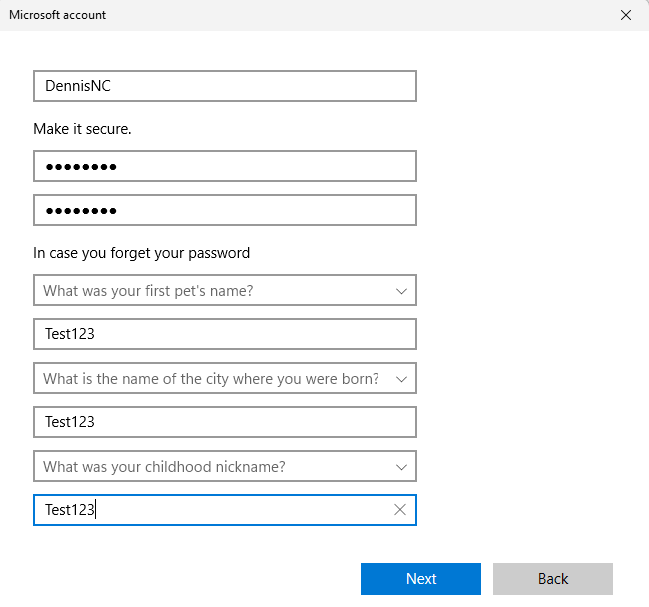
\includegraphics[width=0.99\linewidth]{settings-ms_account.png}%
}
\end{minipage}

Het belangrijkste is een gebruikersnaam (Username) en een wachtwoord (Password). De overige 3 vragen zijn er om je te helpen mocht je het wachtwoord voor dit account vergeten zijn. Beter is het om een password-manager te gebruiken om wachtwoorden voor accounts in op te slaan.

Als we het account aangemaakt hebben kunnen we in deze omgeving alleen nog bepalen tot welk account-type deze nieuwe gebruiker behoort. Klik de gebruiker aan en selecteer \textquote{Change account type}. Hier kunnen we selecteren of de gebruiker een Systeembeheerder is of een normale gebruiker.

\begin{minipage}[t]{\linewidth}
\raggedright
\adjustbox{valign=t}{%
	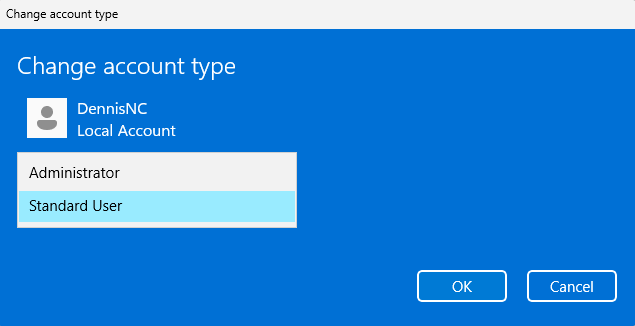
\includegraphics[width=0.99\linewidth]{settings-account_type.png}%
}
\end{minipage}

